\documentclass{homework}
\usepackage{graphicx}

\title{ELEC400m Assignment 3}
\author{Matthew\ Sam}
\date{21/11/2022}

\begin{document}

\maketitle

\exercise

{\Large Part 1 and 2}

Initial 300 epochs on toy data \newline
Best epoch: 298 with loss: 0.11 and acc: 100.00 \newline


\centering
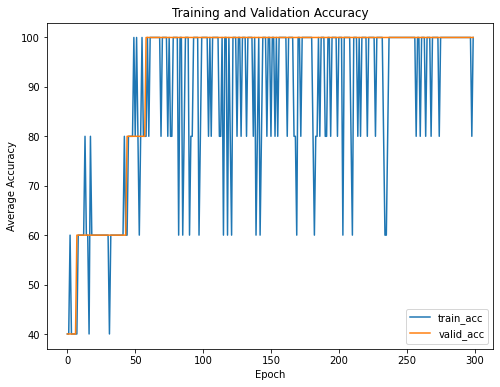
\includegraphics[width=250pt]{accuracyp1.png}

{figure 1: training and validation accuracy}

\raggedright

\centering
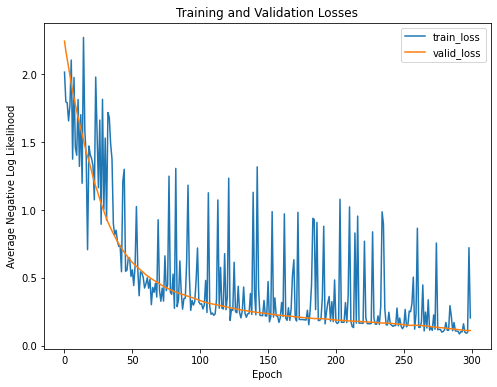
\includegraphics[width=250pt]{lossp1.png}

{figure 2: training and validation loss}

\raggedright

\newpage
\exercise*
{\Large part 3}


30 epochs on MINIST [1,128] \newline
Best epoch: 6 with loss: 0.23 and acc: 94.33 \newline

\centering
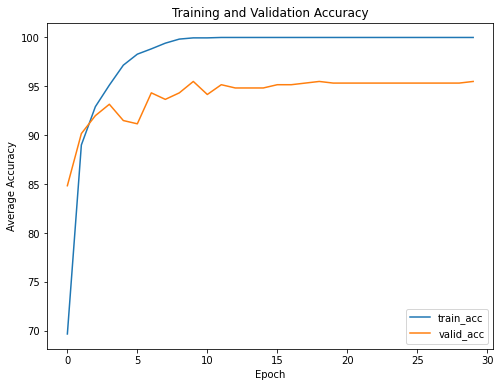
\includegraphics[width=250pt]{accuracyp3_128.png}

{figure 3: training and validation accuracy}

\centering
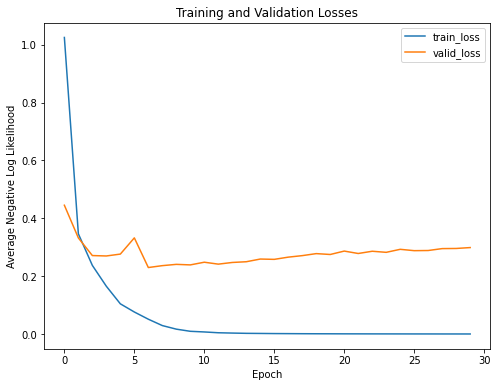
\includegraphics[width=250pt]{lossp3_128.png}

{figure 4: training and validation loss}

\raggedright

\newpage
30 epochs on MINIST [2,512] \newline
Best epoch: 3 with loss: 0.25 and acc: 92.33 \newline

\centering
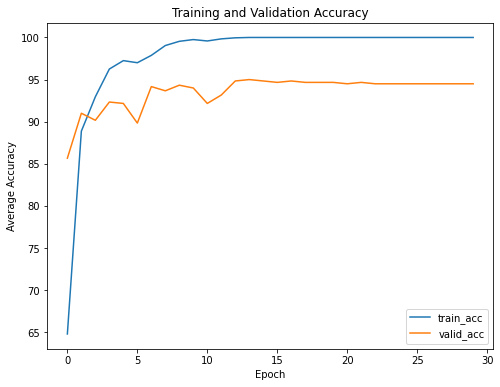
\includegraphics[width=250pt]{accuracyp3_512.png}

{figure 5: training and validation accuracy}

\centering
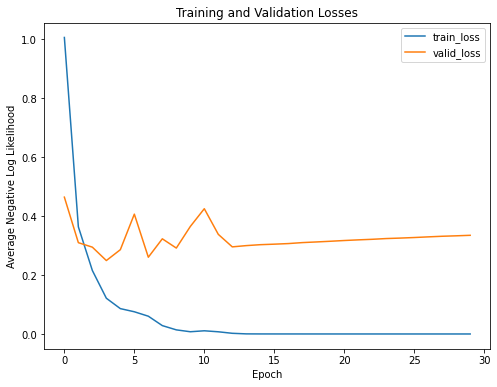
\includegraphics[width=250pt]{lossp3_512.png}

{figure 6: training and validation loss}

\raggedright

\newpage
30 epochs on MINIST [6,5000] \newline
Best epoch: 28 with loss: 0.32 and acc: 93.17 \newline

\centering
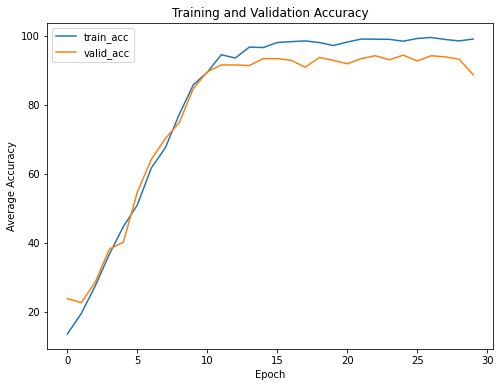
\includegraphics[width=250pt]{accuracyp3_5000.png}

{figure 7: training and validation accuracy}

\centering
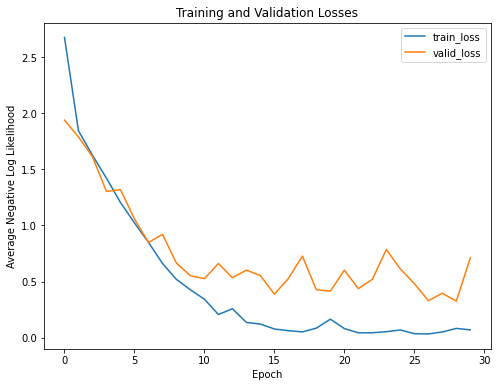
\includegraphics[width=250pt]{lossp3_5000.png}

{figure 8: training and validation loss}

\raggedright

\newpage

\centering
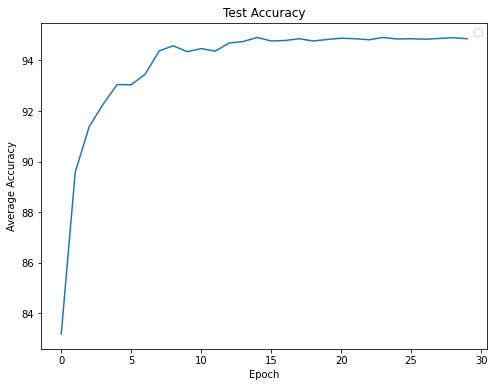
\includegraphics[width=250pt]{Testdata_accuracy.png}

{figure 3: Test data accuracy using sequential number 1}

\centering
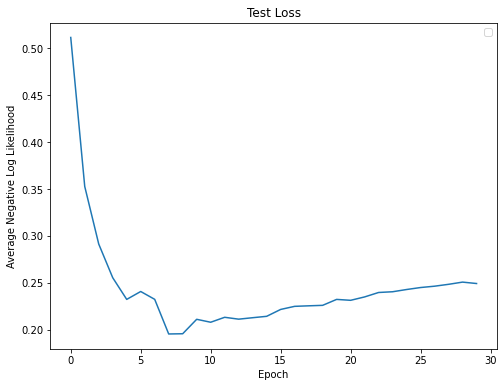
\includegraphics[width=250pt]{testdata_loss.png}

{figure 4: Test data loss using sequential number 1}

\raggedright

\end{document}
